\documentclass[10pt,a4paper]{article}
\usepackage[latin1]{inputenc}
\usepackage[english]{babel}
\usepackage{amsmath}
\usepackage{amsfonts}
\usepackage{amssymb}
\usepackage{makeidx}
\usepackage{graphicx}
\usepackage[left=2cm,right=2cm,top=2cm,bottom=2cm]{geometry}

\author{Anders Dall'Osso Teigset}
\title{Puffer mechanism}

\begin{document}
\maketitle
%Summary
\section{Summary}
\tableofcontents
\newpage
\section{Introduction}
Upon till now SF$_6$ and vacuum based technology have been dominating the compact medium-voltage switchgear market. Air insulated switchgear does exists but they are space consuming and are not applicable for use in a compact substation design. A compact substation is one of the most common designs for substations in the medium-voltage level of the distribution system. Figure \ref{fig:compact substation} displays a compact substation which can be used in the medium-voltage distribution system. As figure \ref{fig:compact substation} displays there is a limited amount of space available for the switchgear. Therefore the main challenge for a air insulated switchgear design for this kind of application is set by the amount of space available in the compact substation. 

\begin{figure} [h]
\centering
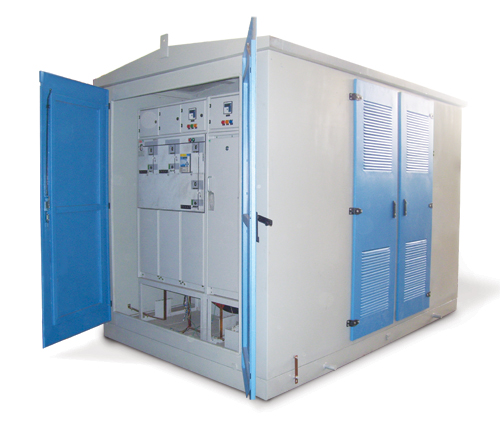
\includegraphics[scale=0.5]{Bilder/Introduction/general_substation.jpg}
\caption{Compact substation with open front panel} \label{fig:compact substation}
\end{figure}



The main choice of interrupting media in switchgear has been SF$_6$ since its discovery in the 1970ies. The production costs of the switchgear is low and the gas is cheap. The gas also have a good dielectric strength, when compared to air it is approximately three times stronger. It has also good thermal conductivity for interrupting currents. The stable form of the gas is not poisonous to humans and it is also not reactive. This means that the gas will not react with other parts of the switchgear and damage it over time. However SF$_6$ have one disadvantaged which have made it less interesting lately. SF$_6$ has $20000$ the greenhouse gas potential as CO$_2$. Due to the development of awareness about the potential threat of global warming phasing out SF$_6$ based equipment where possible is expected to be of interest, both for the government and from many of the larger companies. Klimakur2020 states that:"BLA BLA BLA SF6 SKAL UT"
\end{document}